\documentclass[../thesis.tex]{subfiles}
\begin{document}
\chapter{Single Carrier Device Modeling}\label{sec:polaron_density_measurement}

% this is demonstrated on 17/1/6 in my slides from 17/1/9

\begin{figure}[ht]
\centering
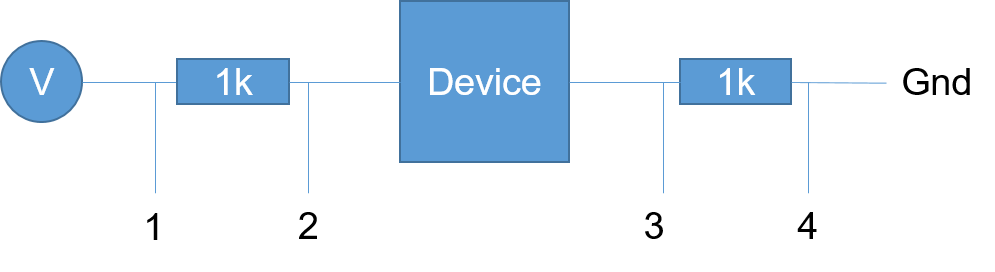
\includegraphics[width=.8\textwidth]{singleCarrier/polaron_circuit}
\caption{Circuit used for measuring polaron density.  Voltage readings are taken at 1-4 overs a 1M$\Omega$ termination.}
\label{fig:polaron_circuit}
\end{figure}

When trying to understand device behavior, it is often important to investigate single carrier devices to understand one charge species at a time or isolate dynamic processes.
An example of this is measurement of the triplet-polaron quenching rate constant, demonstrated in Chapter \ref{sec:pl_measurements}.
Determination of the polaron density is often critical in order to quantify these results.
This is often done by assuming the device is operating within the space charge limit, in which charges have overcome injection barrier limits and transport through the bulk of the material is the limiting process.\cite{Reineke2007,Erickson2014}
In the space-charge limit, current is most simply described using the Mott-Gurney Law, and can be modified to include various trap states to adapt to different semiconductor properties.\cite{Pope1999}
However, space-charge limited current is really only accurate for device behavior at high voltages for thick devices.  
Often, organic layer stacks of interest feature relatively thin layers, and voltages close to the injection limits.
It can be difficult to identify when a device is operating in the space-charge limit.

In order to reduce some of the uncertainty associated with determining polaron density, a differential current measurement can be conducted.  
For a single carrier device, only one type of carrier is injected.  
As charge is being injected into the device and a steady-state polaron density is being achieved, the current on the side of the device where charges are injected should be greater than on the other side.
This can be seen in Figure \ref{fig:polaron_circuit}, where for a hole only device, the current over $R_{12}$ should be greater than the current over $R_{34}$.
All of these signals can be measured using an oscilloscope.
Once steady-state is achieved, the currents should be equal.
The polaron population injected into the device can be calculated using the following equation

\begin{equation}
N_{pol}=\int frac{J_{1-2}-J_{3-4}}{e}dt
\label{eqn:polaron_population_calculation}
\end{equation}

\begin{figure}[ht]
\centering
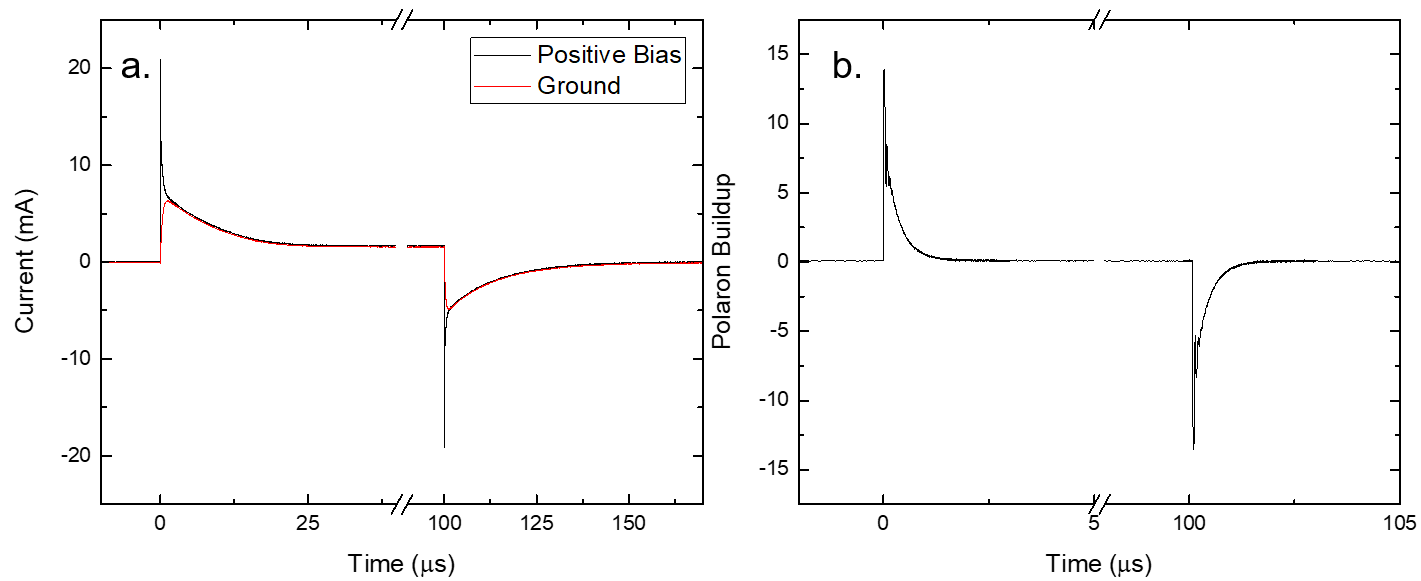
\includegraphics[width=.8\textwidth]{singleCarrier/differential_currents}
\caption{Differential currents for a hole only device. Currents on either side of the device are shown in a. while the difference between them is shown in b.}
\label{fig:differential_currents}
\end{figure}

where $J$ is the current and 1-4 are labeled in Figure \ref{fig:polaron_circuit}.
When voltage is removed from the device, the currents will diverge and the polaron density will be drained from the device.
This is demonstrated in Figure \ref{fig:differential_currents}, with the currents on either side of the device and the differential current shown in \ref{fig:differential_currents}a and \ref{fig:differential_currents}b, respectively.
Notice the positive differential when current is applied and polarons enter the device, and negative when they are removed.

\begin{wrapfigure}{r}{.5\textwidth}
    \begin{minipage}{\linewidth}
    \centering%\captionsetup[subfigure]{justification=centering}
    \begin{subfigure}{.24\textwidth}
    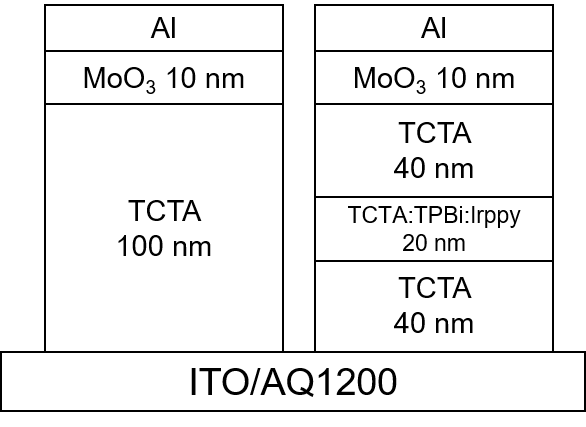
\includegraphics[width=0.48\textwidth]{singleCarrier/SC_architectures}
    \caption{}
    \label{fig:SC_architectures}\par\vfill
    \end{subfigure}

    \begin{subfigure}{.24\textwidth}
    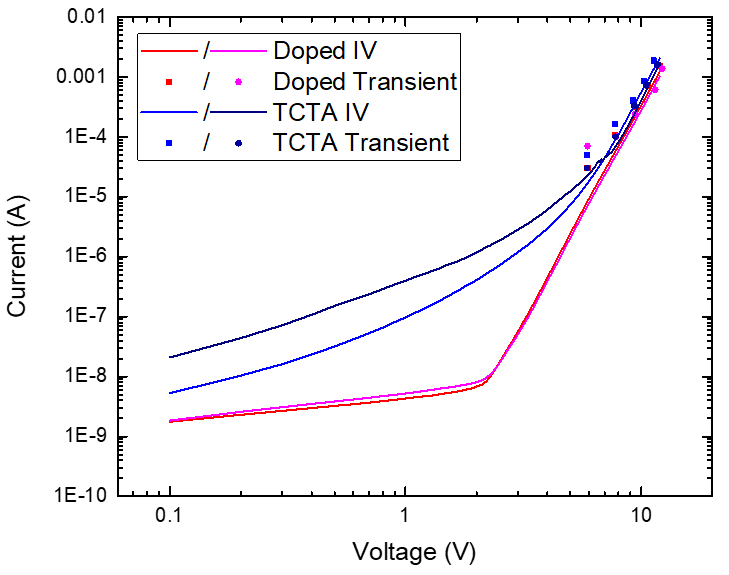
\includegraphics[width=0.48\textwidth]{singleCarrier/SC_ivs}
    \caption{}
    \label{fig:SC_ivs}
    \end{subfigure}
\end{minipage}
\caption{a. Hole only device architectures. b. Current Voltage characteristics for the devices shown in a.  Steady-state sweeps as well as current measured from the differential technique are shown.}
\end{wrapfigure}

While this technique is able to accurately tell the injected polaron population, the distribution of that population is still unknown.
This technique does provide the advantage that with the total polaron population known, the current or voltage dependence of the population can be compared to different models to further validate the operational regime.
Then, a model can be applied to show the spatial dependence of charge.\cite{Pope1999,Mark1962,Lampert2002a}
This technique has the advantage that only the spatial dependence is needed, rather than having to estimate the total charge population, and is more accurate than previous methods relying on solely modeling.

\begin{wrapfigure}{r}{.5\textwidth}
    \centering%\captionsetup[subfigure]{justification=centering}
    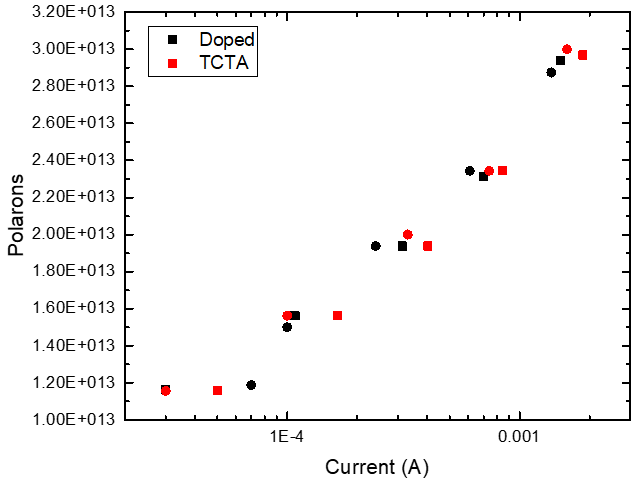
\includegraphics[width=0.48\textwidth]{singleCarrier/SC_polaron_pop_vs_current}
    %\subcaption{}
    \caption{Polaron population as a function of current for the devices in Figure \ref{fig:SC_architectures}}
    \label{fig:SC_polaron_densities}
\end{wrapfigure}

Ideally the polaron population can be restriced to a small area of the device to minimize the extent of the spatial distribution.  
To achieve this, the devices shown in Figure \ref{fig:SC_architectures} were investigated.
The region of interest is the mixed doped layer in the right hand device.
This doped region should show a greater ability to facilitate trapped charge and show a larger polaron population.
The current-voltage profile of these devices is shown in Figure \ref{fig:SC_ivs} where the doped devices show a stronger diode behavior.
The currents obtained from the displacement current measurements show agreement with the steady state current.

The polaron population as a function of current is shown for these devices in Figure \ref{fig:SC_polaron_densities}.
Unfortunately, polaron populations for both devices are almost identical and the hypothesis of increased trapping in the doped region is not correct.
This means that charges are not confined and there is likely a wide distribution of the polaron density.
Despite these drawbacks, the polaron population is still obtained and can be compared to space-charge limited current models.

\section{Future Work}

This techique is useful for a variety of techniques where polaron population needs to be known precisely.
One ready application of this technique is for triplet-polaron quenching measurements.
As discussed in Chapter \ref{sec:pl_measurements}, measurement of \ktp relies on optically pumping a single carrier device under an applied current.
To accurately determine the constant, the polaron density must be known precisely.
The differential current technique would be useful for comparing different materials and their values of \ktp.
Another application with similar motivations would be the optical degradation of single carrier devices.  

Differential current analysis of single carrier devices provides a straight forward way of determining the polaron population within a single carrier device.
While the spatial distribution of the polaron population may not be known, this can be easily modeled with the current dependence of the polaron population available for validation of the model.
Though so far unused in a relevant application, this technique allows more sophisticated comparison of devices when matched polaron population is important.









\ifcsdef{mainfile}{}{\bibliography{../library}}
\end{document}
